\documentclass[10pt]{article}

\usepackage[pdftex]{graphicx}% Adds the ability to include images 
\usepackage[margin=2.5cm, top=1cm, a4paper]{geometry}
\usepackage[T1]    {fontenc }% Allow accented output charachters
\usepackage[utf8]  {inputenc}% Allow accented input charachters 
\usepackage    {xcolor   }% Colors are fun :)
\usepackage{array}
\usepackage        {lmodern }% Modern output font 
\usepackage{amsmath,amssymb,latexsym}
\usepackage{fancyhdr}
\setlength{\headheight}{20pt}
\usepackage{sectsty}
\usepackage{hyperref} 
\usepackage{dashrule}
\usepackage{graphicx}

\definecolor{lightgray}{gray}{0.8}

\newcolumntype{L}{>{\raggedleft}p{0.14\textwidth}}
\newcolumntype{R}{p{0.8\textwidth}}
\newcommand\VRule{\color{lightgray}\vrule width 0.5pt}

\pagestyle{fancy}
\fancyhead{}
\fancyfoot{}
\fancyfoot[C]{\emph{Gábor Bernát}\\\thepage}
\fancyfoot[RO, LE] {bernat@primeranks.net}
\fancyfoot[LO, RE] {$+36$--$30$--$522$--$0450$}
\renewcommand{\headrulewidth}{0pt}

\sectionfont{\fontsize{12}{15}\selectfont}
\newcolumntype{R}[1]{>{\raggedleft\arraybackslash}m{#1}}

\newcommand{\twoColumns}[2]{
  \noindent\begin{tabular}{ p{31em}  R{12.5em} }
    #2 & \emph{#1} \\
\end{tabular}
}
\newcommand{\localsep}{\noindent\hdashrule[0.5ex]{46em}{1pt}{4pt}}

\begin{document}

\begin{minipage}{0.65\textwidth}
\begin{center}
\textbf{\Huge{\MakeUppercase{Gábor Bernát}}}\\
\baselineskip=0pt
\begin{alignat*}{100}
\mbox{+}36\mbox{--}30\mbox{--}522\mbox{--}0450 \mbox{\hspace{0.1cm}}  &\Diamond \mbox{\hspace{0.1cm}bernat@primeranks.net} \\
\mbox{Róna utca } 105\mbox{.\ A/} 12               \mbox{\hspace{0.1cm}} &\Diamond \mbox{\hspace{0.1cm}Budapest, Hungary, } 1145 
\end{alignat*}
\end{center}
\end{minipage}
\begin{minipage}{0.25\textwidth}
\flushright{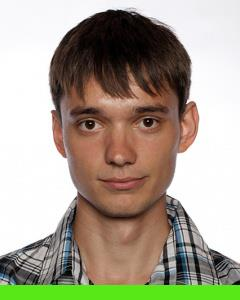
\includegraphics[width=2.5cm]{img/foto.jpg}}
\end{minipage}

\section*{\MakeUppercase{Summary}}
\leaders\vrule width \textwidth\vskip0.3pt % or other desired thickness
\vskip\medskipamount % 

Gábor (surname) Bernát (first name) is a young software engineer believer of the polyglot
programming, currently working full time in Budapest at the ,,Gravity -- Rock solid 
recommendations'' integration engineer. Finished recently his master studies with 
outstanding results in the domain of computer science. 


Amassed throughout the years vast theoretical and practical knowledge base in areas such as 
software development, recommendation enginees, operational tasks, data science, CAD, computer 
vision, mobile robots, and etcetera. He is also a conscious self-driven learner and performer
having written multiple technical articles in various domains of the IT. Sample codes and reports
from projects participated in may be found at \emph{http://primeranks.net/yeti/Work/Portofolio} or at \emph{https://github.com/gaborbernat}.

\section*{\MakeUppercase{Experience}}
\leaders\vrule width \textwidth\vskip0.3pt % or other desired thickness
\vskip\medskipamount % 

\twoColumns{2011 September--on going}{ \textbf{Gravity Research \& Development} }
\twoColumns{Budapest, Hungary}{ \emph{Integration and software engineer} }

The company provides hundred millions of recommendations on a Software--as--a--Service platform
on a daily basis to clients such as rci\@.com, livejasmin\@.com, ivi\@.ru, 
vatera\@.hu and etcetera. Analyzing customer systems; planning, overviewing and doing the integration of them with the 
recommendation platform.Planning and implementing various internal systems to help with the 
integration flow and customer experience (bash shell \& python scripts, PHP \& JavaScript based 
reporting web page). Programming and maintaining a recommendation engine demo application (\@.NET \& Silverlight).

\localsep
\vskip\bigskipamount % 

\twoColumns{2011 May--August}{ \textbf{OpenCV (Open Source Computer Vision Library)} }
\twoColumns{Târgu Mureş, Romania}{ \emph{Technical writer and programmer (part of Google Summer of Code 2011)} }

Learned and used the reStructuredText documentation system to create various tutorials for the OpenCV 
library in both HTML and PDF output format. Helping to architect and create the system used for the 
docummendation, as well co-supervisoring another person on the project. You can view the end result here: 
\emph{http://docs.opencv.org/doc/tutorials/tutorials.html}.

\localsep

\twoColumns{2007 - 2010}{ \textbf{Ziff Davis Enterprise – The DevShed Network}}
\twoColumns{HQ: Fort Lauderdale, USA}{ \emph{Technical writerer} }

Writing articles with technical content on various fields of IT including both introductory and advanced 
techniques for programmers, hardware component reviews and various internet/computer usage tips.
All the articles are published in one of the $13+$ technology websites of the company.
I have multiple articles written about C/C$++$, coding styles, and so forth that are number one
in the Google search and have a \textasciitilde$65,000+$ unique views. You can obtain a full list of them at
\emph{http://primeranks.net/php/articles.php}.

\localsep

\twoColumns{January 2010 - April 2010}{ \textbf{Simon Fraser University}}
\twoColumns{Vancouver,Canada}{ \emph{System architect and implementation} }

Coded the image processing and acquisition algorithm (in C/C++ language) for a research whose
ultimate goal is to develop robots that will play hockey on their own with artificial intelligence. Fur-
thermore made the integration of the written code to the .NET environment and developed the user
interface for it in C\#. This was a team effort (of four) and successfully managed to get the system up and running with an
acceptable error rate. The project was port of a student exchange program through what I attended for a semester classes at
the Simon Fraser University in Vancouver, Canada. Gained foreign experience.

\localsep

\twoColumns{October 2007 - Juny 2008}{ \textbf{XData Consulting SRL – http://cadelix\@.ro}}
\twoColumns{Târgu Mureş, Romania}{ \emph{Junior Software Develper} }

Written a registry editor for internal usage (in C++) using the MFC library for user interface.
Created the basic build up (basic geometrical classes, serialization system, interaction/transformation
and drawing of geometrical objects in MFC) for CAD software developed by the company.
Used the C++ template based loki library. Amassed working experience and techniques at a professional company.

\section*{\MakeUppercase{Education}}
\leaders\vrule width \textwidth\vskip0.3pt % or other desired thickness
\vskip\medskipamount % 

\twoColumns{2011 September--2013 June}{ \textbf{Budapest University of Technology and Economics, Hungary.} } 
\twoColumns{}{Master's degree in Engineering Information Technologist. }

Major in \emph{applied informatics} (grade $4.57/5$ -- excelent). Thesis: ,,Analysis of data mining and 
recommendation services: open source solutions on a scalable framework'', url: http://goo.gl/kwudG2.

\localsep

\twoColumns{2007 September--2011 June}{ \textbf{Sapientia -- Hungarian University of Transylvania, Romania.} } 
\twoColumns{}{Bachelor's degree in Computer Science (grade $9.70/10$).}

Thesis: ,,Regional segmentation of images with B--Spline level set models'', url: http://goo.gl/8nCz9S.

\section*{\MakeUppercase{Technical strengths}}
\leaders\vrule width \textwidth\vskip0.3pt % or other desired thickness
\vskip\medskipamount % 

\begin{tabular}{l p{32em}}
  \textbf{Computer languages}  & C/C$++$, C\#, \emph{Java}, \emph{Python}, Bash, JavaScript, CSS, HTML, R, LaTex, reStructuredText, PHP\\ 
  \textbf{Protocols and apis}  & XML, JSON, REST, jQuery, Qt, SqlAlchemy, ggplot\\
  \textbf{Databases}           & MySQL (Percona), basic of Cassandra, Hadoop (HBase), Redis  \\
  \textbf{Tools}               & git, vim, tmux, Eclipse, Netbeans, Intellij IDEA, Visual Studio, RStudio, Maven, Gradle,
                                 IPython, SQuirreL SQL Client, JIRA, Confluence\\
\end{tabular}
\end{document}
